\documentclass[11pt,addpoints,answers]{exam}
%% This template uses the exams class 
%% Use answers argument only for the model solution.

%%%%%%%%% DeptEEE Standard LaTeX Template Starts Here %%%%%%%%%
%%%%%%%% Based on Physics version thanks to Dave Dunbar %%%%%%%%


%BEGIN DO NOT EDIT
\input EEERubricImportEnglish2022v1
%END DO NOT EDIT

%Uncomment ones of these lines.
%\dept{Computer Science}
%\dept{Mathematics}
\dept{Electronic and Electrical Engineering}
%\dept{Physics}
%... or - if not one of these depts - add \dept{your dept name}

%Update these values 
\module{ABC123} %<<<<<<<<<< replace ABC123 with your module code
\title{TITLE}          %<<<<<<<<<< replace TITLE with your module title
\session{May-June 2019/2020}           %<<<<<<<<<< replace 2019/2020 with the current academic year

%Update this value - durations should be in HOURS and MINUTES (e.g 1hour 30 min - not 90 min)
\timeallowed{x hours} %<<<<<<<< change x hours to the duration of your exam


%These lines control information on  dictionaries calculators and open book exams - uncomment as required
% FOR CLOSED BOOK EXAMS WITH NOT CALCULATORS WHICH ALLOW ENGLISH/WELSH DICTIONARIES,
% YOU CAN LEAVE THIS ALL AS IT IS.

%DICTIONARIES
%\englishwelshallowed %<<<<<<<<<  Candidates may only refer to the English and Welsh language dictionaries available  - this is the default
%\englishonly                %<<<<<<<<<  Candidates may only refer to the English dictionaries available
%\providedglossary        %<<<<<<<<<  Pre-prepared individual bilingual glossary may be used
%\translationdict           %<<<<<<<<<  Candidates may use Welsh to/from English translation dictionaries
%\dictnotallowed          %<<<<<<<<<  The use of any dictionary is not allowed

%CALCULATORS
%\nocalculators             %<<<<<<<<<  No calculators are permitted - this is the default
\univcalculators           %<<<<<<<<<  Candidates will be supplied with a UNIVERSITY calculator
%\approvedcalculators    %<<<<<<<<< Candidates may used apporved non-programmable calculators

% OPEN/CLOSED BOOK
%\notopenbook     %<<<<<<<<< The exam is not open book - this is the default
%\openbook          %<<<<<<<<< Exam is open book

% Exam information - e.g. 'Answer x questions from y' - 'Answer all questions' etc.
% if you need italic or bold use \textit{..} and \textbf{...}  NOT  \it or \bf (which will look awful)
\examinformation{None}     %<<< Replace 'none' with your exam information

% Any special instructions 
\specialinstructions{None}  %<<< If you have special instructions, replace 'none' with them

% some users need the following package - you know if it's you  - uncomment if required
\usepackage{amsmath}

%...and add other packages as appropriate here

%BEGIN DO NOT EDIT
\begin{document}
    %% TITLE Page for FSE Exams
% You shouldn't need to edit this for most purposes
\begingroup
%\fontfamily{phv}\selectfont
\begin{figure}[t]
\begin{flushright}
{\includegraphics*[height=3.0truecm]{SULogo.eps}}
% \label{BoxFigure}
\end{flushright}
\end{figure}

\noindent{\normalsize\textbf{{Faculty of Science and Engineering}}}
\vskip 4mm
\noindent{\normalsize{\dept}}
\vskip 4mm
\noindent{\Large{\textbf{\module}}}
\noindent{\oneline{\Large{\textbf{\title}}}}
\vskip 4mm
\noindent{\normalsize\textbf{{\session}}}
\vskip 4mm
\noindent{\normalsize\textbf{{Time Allowed: \duration}}}
\vskip 4mm
\noindent{\textbf{Do NOT turn over your question paper until instructed to do so.}}

\vskip 4mm

\noindent{\textbf{\textit{Exam Paper Information}}}
\vskip 4mm
\begingroup
\examinfo
\endgroup
\vskip 4mm

\noindent{\textbf{\textit{Special Instruction(s)}}}
\vskip 4mm
\begingroup
\specialinfo
\endgroup
\vskip 4mm

\noindent{\textbf{\textit{Specific Items}}}
\begin{itemize}
\item[] {\small{Dictionaries - \dictionaries}}
\item[] {\small{Calculators - \calculator}}
\item[] {\small{Open Book - \open}}
\end{itemize}

\vskip 10mm
\par
\begingroup
\setlength{\parindent}{0pt}
%\BLURB
\endgroup
\newpage
\endinput
 
% END DO NOT EDIT

%
% ENTER ANY ADDITIONAL INSTRUCTIONS THAT CANNOT FIT ON FRONT PAGE HERE
%
% Do NOT put any instructions that invigilators must be aware of anywhere except the 1st page
%
% ENTER TEXT OF PAPER HERE
% Pick a standard, readable font. Advice from Student
% Services is that Sans Serif fonts are more accessible (however, evidence
% does not appear very strong). Exams Office prefers Arial 11.
% It's recognised that this may not be possible/appropriate in all cases

% See the documentation for the [exams class](https://math.mit.edu/~psh/exam/examdoc.pdf) 
% for details of how to use this template

\begin{questions}
    \titledquestion{Title of the question}
    \begin{parts} 
        \part Answer all subparts
        \begin{subparts}%
            \subpart Answer the following:
            \begin{subsubparts}%
                \subsubpart[2] Describe the colour blue.\droppoints
                \begin{solution}
                    That's quite a subjective question which is difficult to answer precisely.
                \end{solution}
            \end{subsubparts}
        \end{subparts}
    \end{parts}
    \droptotalpoints
\end{questions}


% End matter -- e.g. formulae here
\newpage
% Comment out the formulae you don't need or add your own and input them here
\label{formulae}
%% BEGIN  examhand.tex
\def\FileDate{93/11/01}
\def\FileVersion{1.0}
%%
%% COPYRIGHT 1993-2010, by Chris P. Jobling, C.P.Jobling@Swansea.ac.uk
%%
%% Control Systems: Examinations Handout

%% $Id$

\section*{\module\ \title\ -- Formulae for Examination Use}
For ease of reference, this and the following pages may be detatched from the examination paper.

\begin{multicols}{2}
\begin{enumerate}[label=\roman*]
\item \textit{Even signal}: $x(t) = x(-t)$.
\item \textit{Odd signal}: $-x(t) = x(-t)$.
\item \textit{Composition of signal from odd and even components}: 
$x(t) = x_e(t) + x_o(t)$ where $x_e(t) = \left(x(t) + x(-t)\right)/2$ and 
$x_o(t) = \left(x(t) - x(-t)\right)/2$.
\item \textit{Periodic signals}: A signal $x(t)$
is periodic with fundamental frequency $\Omega$ \unit{\radian\per\second} 
when $x(t) = x(t + nT)$ for all $n$ ($n$ is an integer). The fundamental period
$𝑇 = 2\pi/\Omega$ \unit{\second}.
\item \textit{Energy in a signal $x(t)$}: 
$$
E_x = \int_{-\infty}^{\infty} \left|x(t)\right|^2\,dt\quad\unit{\joule}
$$
\item \textit{Average power in a signal $x(t)$}: 
$$
P_x = \lim_{T\to \infty}\frac{1}{T}\int_{-T/2}^{T/2} \left|x(t)\right|^2\,dt\quad\unit{\watt}
$$
\item \textit{Average power in a periodic signal $x(t)=x(t + nT)$}: 
$$
P_x = \frac{1}{T}\int_{0}^{T} \left|x(t)\right|^2\,dt\quad\unit{\watt}
$$
\item \textit{RMS power}: $\mathrm{RMS}_x = \sqrt{P_x}\,\quad\unit{\watt}$
\item \textit{Mean value of a periodic signal $x(t) = x(t + nT)$}: 
$$
  M_x = \frac{1}{T}\int_0^T x(t)\,dt
$$
\item \textit{Crest factor}: $\mathrm{CF}_x = \frac{\left|x_{\mathrm{peak}}\right|}{\mathrm{RMS}_x}$.
\item \textit{Absolute value of a complex number}: $\left|z\right| = \sqrt{zz^*}$
where $z^*$ is the complex conjugate of $z$.
\item \textit{Euler’s identity}:
\begin{align*}
  e^{j\theta} &= \cos{\theta} + j\sin{\theta}\\
  \cos{\theta} &= \frac{1}{2}\left(e^{j\theta}+e^{-j\theta}\right)\\
  \sin{\theta} &= \frac{1}{j2}\left(e^{j\theta}-e^{-j\theta}\right)
\end{align*}
\item \textit{Selected trig. identities}:
\begin{align*}
  \sin^2\theta &= \frac{1}{2}\left(1-\cos{2\theta}\right)\\
  \cos^2\theta &= \frac{1}{2}\left(1+\cos{2\theta}\right)
\end{align*}
\item \textit{Selected integrals}:
\begin{align*}
  \int \cos\theta\,d\theta &= \sin\theta\\
  \int \sin\theta\,d\theta &= - \cos \theta\\
  \int te^{-at}\,dt &= \left(\frac{at + 1}{a^2}\right)e^{-at}
\end{align*}
\item \textit{Integration by parts}:
$$
\int udv = uv + \int vdu
$$
\item \textit{Convolution}:
$$
x(t) * h(t) = \int_{-\infty}^{\infty}x(\tau)h(t - \tau)\,d\tau
$$
\item \textit{Impulse response}: $h(t) = \mathbf{T}\left\{\delta(t)\right\}$ where $\mathbf{T}$ is the system function.
\item \textit{Step response}:
$$
s(t) = h(t)*u_0(t) = \int_0^t h(\tau)\,d\tau
$$
\item \textit{Signum (sign) function}: $\mathrm{sgn}(t) = 2u_0(t) - 1$
\item \textit{Exponential Fourier series}:
\begin{align*}
  X(t) &= \sum_{k = -n}^{n} C_k e^{jk\Omega_0 t}\\
  C_0 &= \frac{1}{T}\int_0^T x(t)\,dt\\
  C_k &= \frac{1}{T}\int_0^T x(t)e^{jk\Omega_0 t}\,dt\\ 
      &= \frac{1}{2\pi}\int_0^{2\pi} x(\theta)e^{jk\theta}\,d\theta
\end{align*}
\item \textit{Trig. Fourier series}:
$$
F(s) = \frac{1}{2}a_0 + \sum_{k=1}^{\infty} \left( a_k \cos k\Omega_0 t + b_k \sin k\Omega_0 t\right)
$$
\item \textit{Trig. Fourier series coefficients from exponential Fourier series coefficients}:
\begin{align*}
  a_0 &= 2C_0\\
  a_k &= C_k + C_{-k}\\
  b_k &= j\left(C_k - C_{-k}\right)
\end{align*}
\item \textit{Parseval's theorem}: 
$$
\frac{1}{T}\int_{-T/2}^{T/2} \left|x(t)\right|^2\, dt = \sum_{k=\infty}^{\infty} \left|C_k\right|^2
$$
\end{enumerate}
\end{multicols}




\endinput













\subsection*{The Complex Frequency Domain}

\subsubsection*{The Laplace Transform}
$$
F(s)=\mathcal{L}\left\{f(t)\right\}=\int_0^{\infty} f(t)e^{-st}\, dt
$$
\subsubsection*{The Inverse Laplace Transform}
$$
f(t)=\mathcal{L}^{-1}\left\{F(s)\right\}=\frac{1}{j2\pi}\int_{\sigma-j\omega}^{\sigma+j\omega} F(s)e^{st}\, ds
$$
\subsubsection*{Laplace Transform Properties}

%% Table of laplace transform properties

\begin{longtable}[]{@{}
    >{\raggedleft\arraybackslash}p{(\columnwidth - 6\tabcolsep) * \real{0.1351}}
    >{\raggedright\arraybackslash}p{(\columnwidth - 6\tabcolsep) * \real{0.2703}}
    >{\raggedright\arraybackslash}p{(\columnwidth - 6\tabcolsep) * \real{0.2162}}
    >{\raggedright\arraybackslash}p{(\columnwidth - 6\tabcolsep) * \real{0.3784}}@{}}
  \toprule\noalign{}
  \begin{minipage}[b]{\linewidth}\raggedleft
  No.
  \end{minipage} & \begin{minipage}[b]{\linewidth}\raggedright
  \textbf{Name}
  \end{minipage} & \begin{minipage}[b]{\linewidth}\raggedright
  \textbf{Time Domain} \(f(t)\)
  \end{minipage} & \begin{minipage}[b]{\linewidth}\raggedright
      \textbf{Complex Frequency Domain} \(F(s)\)
  \end{minipage} \\
  \midrule\noalign{}
  \endhead
  \bottomrule\noalign{}
  \endlastfoot
  1. & Linearity & \(a_1f_1(t)+a_2f_2(t)+\cdots+a_nf_n(t)\) &
  \(a_1F_1(s)+a_2F_2(s)+\cdots+a_nF_n(s)\) \\[3ex]
  2. & Time shifting & \(\displaystyle{f(t-a)}u_0(t-a)\) &
  \(\displaystyle{e^{-a s}F(s)}\) \\[1.5ex]
  3. & Frequency shifting & \(\displaystyle{e^{-as}f(t)}\) &
  \(\displaystyle{F(s+a)}\) \\[1.5ex]
  4. & Time scaling & \(f(a t)\) &
  \(\displaystyle{\frac{1}{a}F\left(\frac{s}{a}\right)}\) \\[1.5ex]
  5. & Time differentiation & \(\displaystyle{\frac{d}{dt}\,f(t)}\) &
  \(\displaystyle{F(s)-f(0^-)}\) \\[1.5ex]
  7. & Frequency differentiation & \(\displaystyle{tf(t)}\) &
  \(\displaystyle{-\frac{d}{ds}F(s)}\) \\[1.5ex]
  8. & Time integration &
  \(\displaystyle{\int_{-\infty}^{t}f(\tau)d\tau}\) &
  \(\displaystyle{\frac{F(s)}{s}+ \frac{F(0^-)}{s}}\) \\[2ex]
  9. & Frequency integration & \(\displaystyle{\frac{f(t)}{t}}\) &
  \(\displaystyle{\int_s^\infty F(\Omega)\,d\Omega}\) \\[2ex]
  10. & Time Periodicity & \(\displaystyle{f(t + nT)}\) &
  \(\displaystyle{\frac{\int_0^T f(t)e^{-st}\,dt}{1 - e^{-sT}}}\) \\[2.5ex]
  11. & Initial value theorem &
  \(\displaystyle{\lim_{t\rightarrow 0} f(t)}\) &
  \(\displaystyle{\lim_{s\rightarrow \infty}sF(s) = f(0^-)}\) \\[1.5ex]
  12. & Final value theorem &
  \(\displaystyle{\lim_{t\rightarrow \infty} f(t)}\) &
  \(\displaystyle{\lim_{s\rightarrow 0}sF(s) = f(\infty)}\) \\[2ex]
  13. & Time convolution & \(\displaystyle{f_1(t)*f_2(t)}\) &
  \(\displaystyle{F_1(s) F_2(s)}\) \\[2ex]
  14. & Frequency convolution & \(\displaystyle{f_1(t)f_2(t)}\) &
      \(\displaystyle{\frac{1}{j2\pi}\left(F_1(s)*F_2(s)\right)} \)\\[2.5ex]
  \end{longtable}
  \endinput

\subsection*{Laplace Transform Pairs}
\label{common-laplace-transform-pairs}

%% Table of Laplace transform paire

\begin{longtable}[]{@{}
    >{\raggedright\arraybackslash}p{(\columnwidth - 6\tabcolsep) * \real{0.1}}
    >{\raggedright\arraybackslash}p{(\columnwidth - 6\tabcolsep) * \real{0.25}}
    >{\raggedright\arraybackslash}p{(\columnwidth - 6\tabcolsep) * \real{0.25}}
    >{\raggedright\arraybackslash}p{(\columnwidth - 6\tabcolsep) * \real{0.25}}@{}}
  \toprule\noalign{}
  \begin{minipage}[b]{\linewidth}\raggedright
  ~
  \end{minipage} & \begin{minipage}[b]{\linewidth}\raggedright
  \(f(t)\)
  \end{minipage} & \begin{minipage}[b]{\linewidth}\raggedright
  \(F(s)\)
  \end{minipage} & \begin{minipage}[b]{\linewidth}\raggedright
  ROC
  \end{minipage} \\
  \midrule\noalign{}
  \endhead
  \bottomrule\noalign{}
  \endlastfoot
  1 & \(\displaystyle \delta(t)\) & \(\displaystyle 1\) & All \(s\) \\[1.5ex]
  2 & \(\displaystyle \delta(t-a)\) & \(\displaystyle e^{-as}\) & All
  \(s\) \\[2ex]
  3 & \(\displaystyle u_0(t)\) & \(\displaystyle \frac{1}{s}\) & Re(\(s\))
  \textgreater{} 0 \\[2ex]
  4 & \(\displaystyle -u_0(-t)\) & \(\displaystyle \frac{1}{s}\) &
  Re(\(s\)) \textless{} 0 \\[2ex]
  5 & \(\displaystyle t u_0(t)\) & \(\displaystyle \frac{1}{s^2}\) &
  Re(\(s\)) \textgreater{} 0 \\[2ex]
  6 & \(\displaystyle t^n u_0(t)\) & \(\displaystyle \frac{n!}{s^{n+1}}\)
  & Re(\(s\)) \textgreater{} 0 \\[2ex]
  7 & \(\displaystyle e^{-at}u_0(t)\) & \(\displaystyle \frac{1}{s+a}\) &
  Re(\(s\)) \textgreater{} \(-\)Re(\(a\)) \\[2ex]
  8 & \(\displaystyle -e^{-at}u_0(-t)\) & \(\displaystyle \frac{1}{s+a}\)
  & Re(\(s\))\textless{} \(-\)Re(\(a\)) \\[1.5ex]
  9 & \(\displaystyle t^n e^{-at} u_0(t)\) &
  \(\displaystyle \frac{n!}{(s+a)^{n+1}}\) & Re(\(s\)) \textgreater{}
  \(-\)Re(\(a\)) \\[3ex]
  10 & \(\displaystyle -t^n e^{-at} u_0(-t)\) &
  \(\displaystyle \frac{n!}{(s+a)^{n+1}}\) & Re(\(s\)) \textless{}
  \(-\)Re(\(a\)) \\[3ex]
  11 & \(\displaystyle \sin (\omega t) u_0(t)\) &
  \(\displaystyle \frac{\omega}{s^2 + \omega^2}\) & Re(\(s\))
  \textgreater{} 0 \\[2.5ex]
  12 & \(\displaystyle \cos (\omega t) u_0(t)\) &
  \(\displaystyle \frac{s}{s^2 + \omega^2}\) & Re(\(s\)) \textgreater{}
  0 \\[2.5ex]
  13 & \(\displaystyle e^{-at} \sin (\omega t) u_0(t)\) &
  \(\displaystyle \frac{\omega}{(s + a)^2 + \omega^2}\) & Re(\(s\))
  \textgreater{} \(-\)Re(\(a\)) \\[2.5ex]
  14 & \(\displaystyle e^{-at}\cos (\omega t) u_0(t)\) &
  \(\displaystyle \frac{s+a}{(s+a)^2 + \omega^2}\) & Re(\(s\))
  \textgreater{} \(-\)Re(\(a\)) \\[2.5ex]
  \end{longtable}
  \endinput

\noindent Notes: ROC = region of convergence. The appearance of $u_0(t)$ in the values shown in the $f(t)$
column ensure that the signals and/or systems that they represent are causal.

\subsection*{The Frequency Domain}

\subsubsection*{The Fourier Transform}

$$
F(j\omega) = \mathcal{F}\left\{f(t)\right\} = \int_{-\infty}^{\infty} f(t)e^{-j\omega t}\,dt
$$

\subsubsection*{The Inverse Fourier Transform}

$$
f(t) = \mathcal{F}^{-1}\left\{F(s)\right\} = \int_{-\infty}^{\infty} F(s)e^{j\omega t}\,dt
$$


\subsubsection*{Properties of the Fourier Transform}

%% Properties of the Fourier transform

\begin{longtable}[]{@{}
  >{\raggedleft\arraybackslash}p{(\columnwidth - 8\tabcolsep) * \real{0.1000}}
  >{\raggedright\arraybackslash}p{(\columnwidth - 8\tabcolsep) * \real{0.2000}}
  >{\raggedright\arraybackslash}p{(\columnwidth - 8\tabcolsep) * \real{0.200}}
  >{\raggedright\arraybackslash}p{(\columnwidth - 8\tabcolsep) * \real{0.20}}
  >{\raggedright\arraybackslash}p{(\columnwidth - 8\tabcolsep) * \real{0.3}}@{}}
\toprule\noalign{}
\begin{minipage}[b]{\linewidth}\raggedleft
No.
\end{minipage} & \begin{minipage}[b]{\linewidth}\raggedright
\textbf{Property}
\end{minipage} & \begin{minipage}[b]{\linewidth}\raggedright
\(f(t)\)
\end{minipage} & \begin{minipage}[b]{\linewidth}\raggedright
\(F(j\omega)\)
\end{minipage} & \begin{minipage}[b]{\linewidth}\raggedright
\textbf{Remarks}
\end{minipage} \\
\midrule\noalign{}
\endhead
\bottomrule\noalign{}
\endlastfoot
1. & Linearity & \(a_1f_1(t)+a_2f_2(t)+\cdots+a_nf_n(t)\) &
\(a_1F_1(j\omega)+a_2F_2(j\omega)+\cdots+a_nF_n(j\omega)\) & Fourier
transform is a linear operator. \\
2. & Symmetry & \(2\pi f(-j\omega)\) & \(F(t)\) & \\
3. & Time and frequency scaling & \(f(\alpha t)\) &
\(\displaystyle{\frac{1}{\lvert\alpha\rvert}F\left(j\frac{\omega}{\alpha}\right)}\)
& time compression is frequency expansion and \emph{vice versa} \\
4. & Time shifting & \(\displaystyle{f(t-t_0)}\) &
\(\displaystyle{e^{-j\omega t_0}F(j\omega)}\) & A time shift corresponds
to a phase shift in frequency domain \\
5. & Frequency shifting & \(\displaystyle{e^{j\omega_0 t}f(t)}\) &
\(\displaystyle{F(j\omega-j\omega_0)}\) & Multiplying a signal by a
complex exponential results in a frequency shift. \\
6. & Time differentiation & \(\displaystyle{\frac{d^n}{dt^n}\,f(t)}\) &
\(\displaystyle{(j\omega)^nF(j\omega)}\) & \\
7. & Frequency differentiation & \(\displaystyle{(-jt)^n f(t)}\) &
\(\displaystyle{\frac{d^n}{d\omega^n}F(j\omega)}\) & \\
8. & Time integration &
\(\displaystyle{\int_{-\infty}^{t}f(\tau)d\tau}\) &
\(\displaystyle{\frac{F(j\omega)}{j\omega}+\pi F(0)\delta(\omega)}\)
& \\[3ex]
9. & Conjugation & \(\displaystyle{f^*(t)}\) &
\(\displaystyle{F^*(-j\omega)}\) & \\[2ex]
10. & Time convolution & \(\displaystyle{f_1(t)*f_2(t)}\) &
\(\displaystyle{F_1(j\omega) F_2(j\omega)}\) & Compare with Laplace
Transform \\
11. & Frequency convolution & \(\displaystyle{f_1(t)f_2(t)}\) &
\(\displaystyle{\frac{1}{2\pi}F_1(j\omega)*F_2(j\omega)}\) & This has
application to amplitude modulation. \\[4ex]
12. & Area under \(f(t)\) &
\(\displaystyle{\int_{-\infty}^{\infty} f(t)\,dt = F(0)}\) & & Way to
calculate DC (or average) value of a signal \\[3ex]
13. & Area under \(F(j\omega)\) &
\(\displaystyle{f(0) = \frac{1}{2\pi}\int_{-\infty}^{\infty}F(j\omega)\,d\omega}\)
& & \\[3ex]
14. & Energy-Density Spectrum &
\(\displaystyle{E_{[\omega_1,\omega_2]}:=\displaystyle{\frac{1}{2\pi}\int_{\omega_1}^{\omega_2}\lvert F(j\omega)\rvert ^2\,d\omega.}}\)
& & \\
15. & Parseval's theorem &
\(\displaystyle{\int_{-\infty}^{\infty}\lvert f(t)\rvert^2\,dt=\displaystyle{\frac{1}{2\pi}\int_{-\infty}^{\infty}\lvert F(j\omega)\rvert ^2\,d\omega.}}\)
& & Definition of RMS follows from this \\[4ex]
\end{longtable}

\endinput


\subsection*{Fourier Transform Pairs}

%% Fourier transform table

\begin{longtable}[]{@{}
  >{\raggedright\arraybackslash}p{(\columnwidth - 8\tabcolsep) * \real{0.0400}}
  >{\raggedright\arraybackslash}p{(\columnwidth - 8\tabcolsep) * \real{0.2}}
  >{\raggedright\arraybackslash}p{(\columnwidth - 8\tabcolsep) * \real{0.2}}
  >{\raggedright\arraybackslash}p{(\columnwidth - 8\tabcolsep) * \real{0.3}}
  >{\raggedright\arraybackslash}p{(\columnwidth - 8\tabcolsep) * \real{0.3}}@{}}
\toprule\noalign{}
\begin{minipage}[b]{\linewidth}\raggedright
No.\end{minipage} & \begin{minipage}[b]{\linewidth}\raggedright
\textbf{Name}
\end{minipage} & \begin{minipage}[b]{\linewidth}\raggedright
\(f(t)\)
\end{minipage} & \begin{minipage}[b]{\linewidth}\raggedright
\(F(j\omega)\)
\end{minipage} & \begin{minipage}[b]{\linewidth}\raggedright
\textbf{Remarks}
\end{minipage} \\
\midrule\noalign{}
\endhead
\bottomrule\noalign{}
\endlastfoot
1. & Dirac delta & \(\delta(t)\) & \(1\) & Constant energy at \emph{all}
frequencies. \\
2. & Time sample & \(\delta(t-t_0)\) & \(e^{-j\omega t_0}\) & \\[1.5ex]
3. & Phase shift & \(e^{j\omega_0 t}\) &
\(2\pi\delta(\omega - \omega_0)\) & \\[3ex]
4. & \emph{Signum} & \(\operatorname{sgn} t\) &
\(\displaystyle{\frac{2}{j\omega}}\) & also known as sign function \\[3ex]
5. & Unit step & \(u_0(t)\) &
\(\displaystyle{\frac{1}{j\omega}+\pi\delta(\omega)}\) & \\[3ex]
6. & Cosine & \(\cos \omega_0 t\) &
\(\pi\left[\delta(\omega-\omega_0)+\delta(\omega+\omega_0)\right]\) & \\[2ex]
7. & Sine & \(\sin \omega_0 t\) &
\(-j\pi\left[\delta(\omega-\omega_0)-\delta(\omega+\omega_0)\right]\)
& \\[2ex]
8. & Single pole & \(e^{-at}u_0(t)\) &
\(\displaystyle{\frac{1}{j\omega + a}}\) & \(a > 0\) \\[3ex]
9. & Double pole & \(te^{-at}u_0(t)\) &
\(\displaystyle{\frac{1}{(j\omega + a)^2}}\) & \(a > 0\) \\[3ex]
10. & Complex pole (cosine component) &
\(e^{-at}\cos \omega_0 t\;u_0(t)\) &
\(\displaystyle{\frac{j\omega + a}{(j\omega + a)^2+\omega_0^2}}\) &
\(a >0\) \\[3ex]
11. & Complex pole (sine component) &
\(e^{-a t}\sin \omega_0 t\;u_0(t)\) &
\(\displaystyle{\frac{\omega}{(j\omega + a)^2+\omega_0^2}}\) &
\(a >t 0\) \\[3ex]
\end{longtable}

\endinput


Notes: The appearance of $u_0(t)$ in the values shown in the $f(t)$ column ensure that 
the signals and/or systems that they represent are causal.
    
\endinput

\subsection*{The Discrete-Time Domain}
\subsubsection*{The Z-Transform}

$$
F(z) = \mathcal{Z}\left\{f[n]\right\} = \sum_{n=0}^{\infty} f[n]z^{-n}
$$

\subsubsection*{The Inverse Z-Transform}

$$
f[n] = \mathcal{Z}^{-1}\left\{F[z]\right\} = \frac{1}{j2\pi}\oint F(z)z^{k-1}\,dz 
$$

\subsubsection*{Properties of the Z-Transform}

%% Table of Z-transform properties

\begin{longtable}[]{@{}
  >{\raggedright\arraybackslash}p{(\columnwidth - 6\tabcolsep) * \real{0.0375}}
  >{\raggedright\arraybackslash}p{(\columnwidth - 6\tabcolsep) * \real{0.3}}
  >{\raggedright\arraybackslash}p{(\columnwidth - 6\tabcolsep) * \real{0.25}}
  >{\raggedright\arraybackslash}p{(\columnwidth - 6\tabcolsep) * \real{0.25}}@{}}
\toprule\noalign{}
\begin{minipage}[b]{\linewidth}\raggedright
No.
\end{minipage} & \begin{minipage}[b]{\linewidth}\raggedright
\textbf{Name}
\end{minipage} & \begin{minipage}[b]{\linewidth}\raggedright
$f[n]$
\end{minipage} & \begin{minipage}[b]{\linewidth}\raggedright
$F(z)$
\end{minipage} \\
\midrule\noalign{}
\endhead
\bottomrule\noalign{}
\endlastfoot
1 & Linearity & \(\displaystyle{af_1[n]+bf_2[n]+\cdots}\) &
\(\displaystyle{aF_1(z)+bF_2(z)+\cdots}\) \\[2ex]
2 & Shift of \(\displaystyle{x[n]u_0[n]}\) &
\(\displaystyle{f[n-m]u_0[n-m]}\) & \(\displaystyle{z^{-m}F(z)}\) \\[2ex]
3 & Left shift & \(\displaystyle{f[n-m]}\) &
\(\displaystyle{z^{-m}F(z)+\sum_{n=0}^{m-1}f[n-m]z^{-n}}\) \\[2.5ex]
4 & Right shift & \(\displaystyle{f[n+m]}\) &
\(\displaystyle{z^{m}F(z)+\sum_{n=-m}^{-1}f[n+m]z^{-n}}\) \\[2.5ex]
5 & Multiplication by \(\displaystyle{a^n}\) &
\(\displaystyle{a^nf[n]}\) &
\(\displaystyle{F\left(\frac{z}{a}\right)}\) \\[2ex]
6 & Multiplication by \(\displaystyle{e^{-nsT_s}}\) &
\(\displaystyle{e^{-nsT_s}f[n]}\) &
\(\displaystyle{F\left(e^{sT_s}z\right)}\) \\[2ex]
7 & Multiplication by \(\displaystyle{n}\) & \(\displaystyle{nf[n]}\) &
\(\displaystyle{-z\frac{d}{dz}F(z)}\) \\[2ex]
8 & Multiplication by \(\displaystyle{n^2}\) &
\(\displaystyle{n^2f[n]}\) &
\(\displaystyle{-z\frac{d}{dz}F(z)+z^2\frac{d^2}{dz^2}F(z)}\) \\[2ex]
9 & Summation in time & \(\displaystyle{\sum_{m=0}^{n}f[m]}\) &
\(\displaystyle{\frac{z}{z-1}F(z)}\) \\[2ex]
10 & Time convolution & \(\displaystyle{f_1[n]*f_2[n]}\) &
\(\displaystyle{F_1(z)F_2(z)}\) \\[2ex]
11 & Frequency convolution & \(\displaystyle{f_1[n]f_2[n]}\) &
\(\displaystyle{\frac{1}{j2\pi }\oint {x{F_1}(v){F_2}\left( {\frac{z}{v}} \right)} {v^{ - 1}}dv}\) \\
12 & Initial value theorem &
\(\displaystyle{f[0]=\lim_{z\to\infty}F(z)}\) & \\[2ex]
13 & Final value theorem &
\(\displaystyle{\lim_{n\to\infty}f[n]=\lim_{z\to 1}(z-1)F(z)}\) & \\[2ex]
\end{longtable}
\endinput


\subsubsection*{Z-Transform Pairs}

%% Z-Transform pairs

\begin{longtable}[]{@{}
  >{\raggedright\arraybackslash}p{(\columnwidth - 6\tabcolsep) * \real{0.1067}}
  >{\raggedright\arraybackslash}p{(\columnwidth - 6\tabcolsep) * \real{0.3733}}
  >{\raggedright\arraybackslash}p{(\columnwidth - 6\tabcolsep) * \real{0.2667}}
  >{\raggedright\arraybackslash}p{(\columnwidth - 6\tabcolsep) * \real{0.2533}}@{}}
\toprule\noalign{}
\begin{minipage}[b]{\linewidth}\raggedright
No.
\end{minipage} & \begin{minipage}[b]{\linewidth}\raggedright
f{[}n{]}
\end{minipage} & \begin{minipage}[b]{\linewidth}\raggedright
F(z).
\end{minipage} & \begin{minipage}[b]{\linewidth}\raggedright
\textbf{Region of Convergence}
\end{minipage} \\
\midrule\noalign{}
\endhead
\bottomrule\noalign{}
\endlastfoot
1. & \(\displaystyle{\delta[n]}\) & \(\displaystyle{1}\) & \\[2.5ex]
2 & \(\displaystyle{\delta[n-m]}\) & \(\displaystyle{z^{-m}}\) & \\[2.5ex]
3 & \(\displaystyle{a^nu_0[n]}\) & \(\displaystyle{\frac{z}{z-a}}\) &
\(\mid z \mid > a\) \\[2.5ex]
4 & \(\displaystyle{u_0[n]}\) & \(\displaystyle{\frac{z}{z-1}}\) &
\(\mid z \mid > 1\) \\[2.5ex]
5 & \(\displaystyle{(e^{-anT_s})u_0[n]}\) &
\(\displaystyle{\frac{z}{z-e^{-aT_s}}}\) &
\(\displaystyle{\mid e^{-aT_s}z^{-1} \mid < 1}\) \\[2.5ex]
6 & \(\displaystyle{(\cos naT_s)u_0[n]}\) &
\(\displaystyle{\frac{z^2 - z\cos aT_s}{z^2 -2z\cos aT_s + 1}}\) &
\({ \mid z \mid> 1}\) \\[2.5ex]
7 & \(\displaystyle{(\sin naT_s)u_0[n]}\) &
\(\displaystyle{\frac{z\sin aT_s}{z^2 -2z\cos aT_s + 1}}\) &
\({\mid z \mid > 1}\) \\[2.5ex]
8 & \(\displaystyle{(a^n\cos naT_s)u_0[n]}\) &
\(\displaystyle{\frac{z^2 - az\cos aT_s}{z^2 -2az\cos aT_s + a^2}}\) &
\({\mid z \mid > 1}\) \\[2.5ex]
9 & \(\displaystyle{(a^n\sin naT_s)u_0[n]}\) &
\(\displaystyle{\frac{az\sin aT_s}{z^2 -2az\cos aT_s + a^2}}\) &
\({\mid z \mid > 1}\) \\[2.5ex]
10 & \(\displaystyle{u_0[n]-u_0[n-m]}\) &
\(\displaystyle{\frac{z^m-1}{z^{m-1}(z-1)}}\) & \\[2.5ex]
11 & \(\displaystyle{nu_0[n]}\) & \(\displaystyle{\frac{z}{(z-1)^2}}\)
& \\
12 & \(\displaystyle{n^2u_0[n]}\) &
\(\displaystyle{\frac{z(z+1)}{(z-1)^3}}\) & \\[2.5ex]
13 & \(\displaystyle{[n+1]u_0[n]}\) &
\(\displaystyle{\frac{z^2}{(z-1)^2}}\) & \\[2.5ex]
14 & \(\displaystyle{a^n n u_0[n]}\) &
\(\displaystyle{\frac{az}{(z-a)^2}}\) & \\[2.5ex]
15 & \(\displaystyle{a^n n^2 u_0[n]}\) &
\(\displaystyle{\frac{az(z+a)}{(z-a)^3}}\) & \\[2.5ex]
16 & \(\displaystyle{a^n n[n+1] u_0[n]}\) &
\(\displaystyle{\frac{2az^2}{(z-a)^3}}\) & \\[2.5ex]
\end{longtable}
\endinput

\noindent Notes: The appearance of $u_0[t]$ in the values shown in the $f[t]$ column ensure that 
the signals and/or systems that they represent are causal.
    
\endinput

%% The Discrete Fourier transform

\subsection*{The Discrete Frequency Domain}


    \begin{figure}[htb]
        \begin{center}
            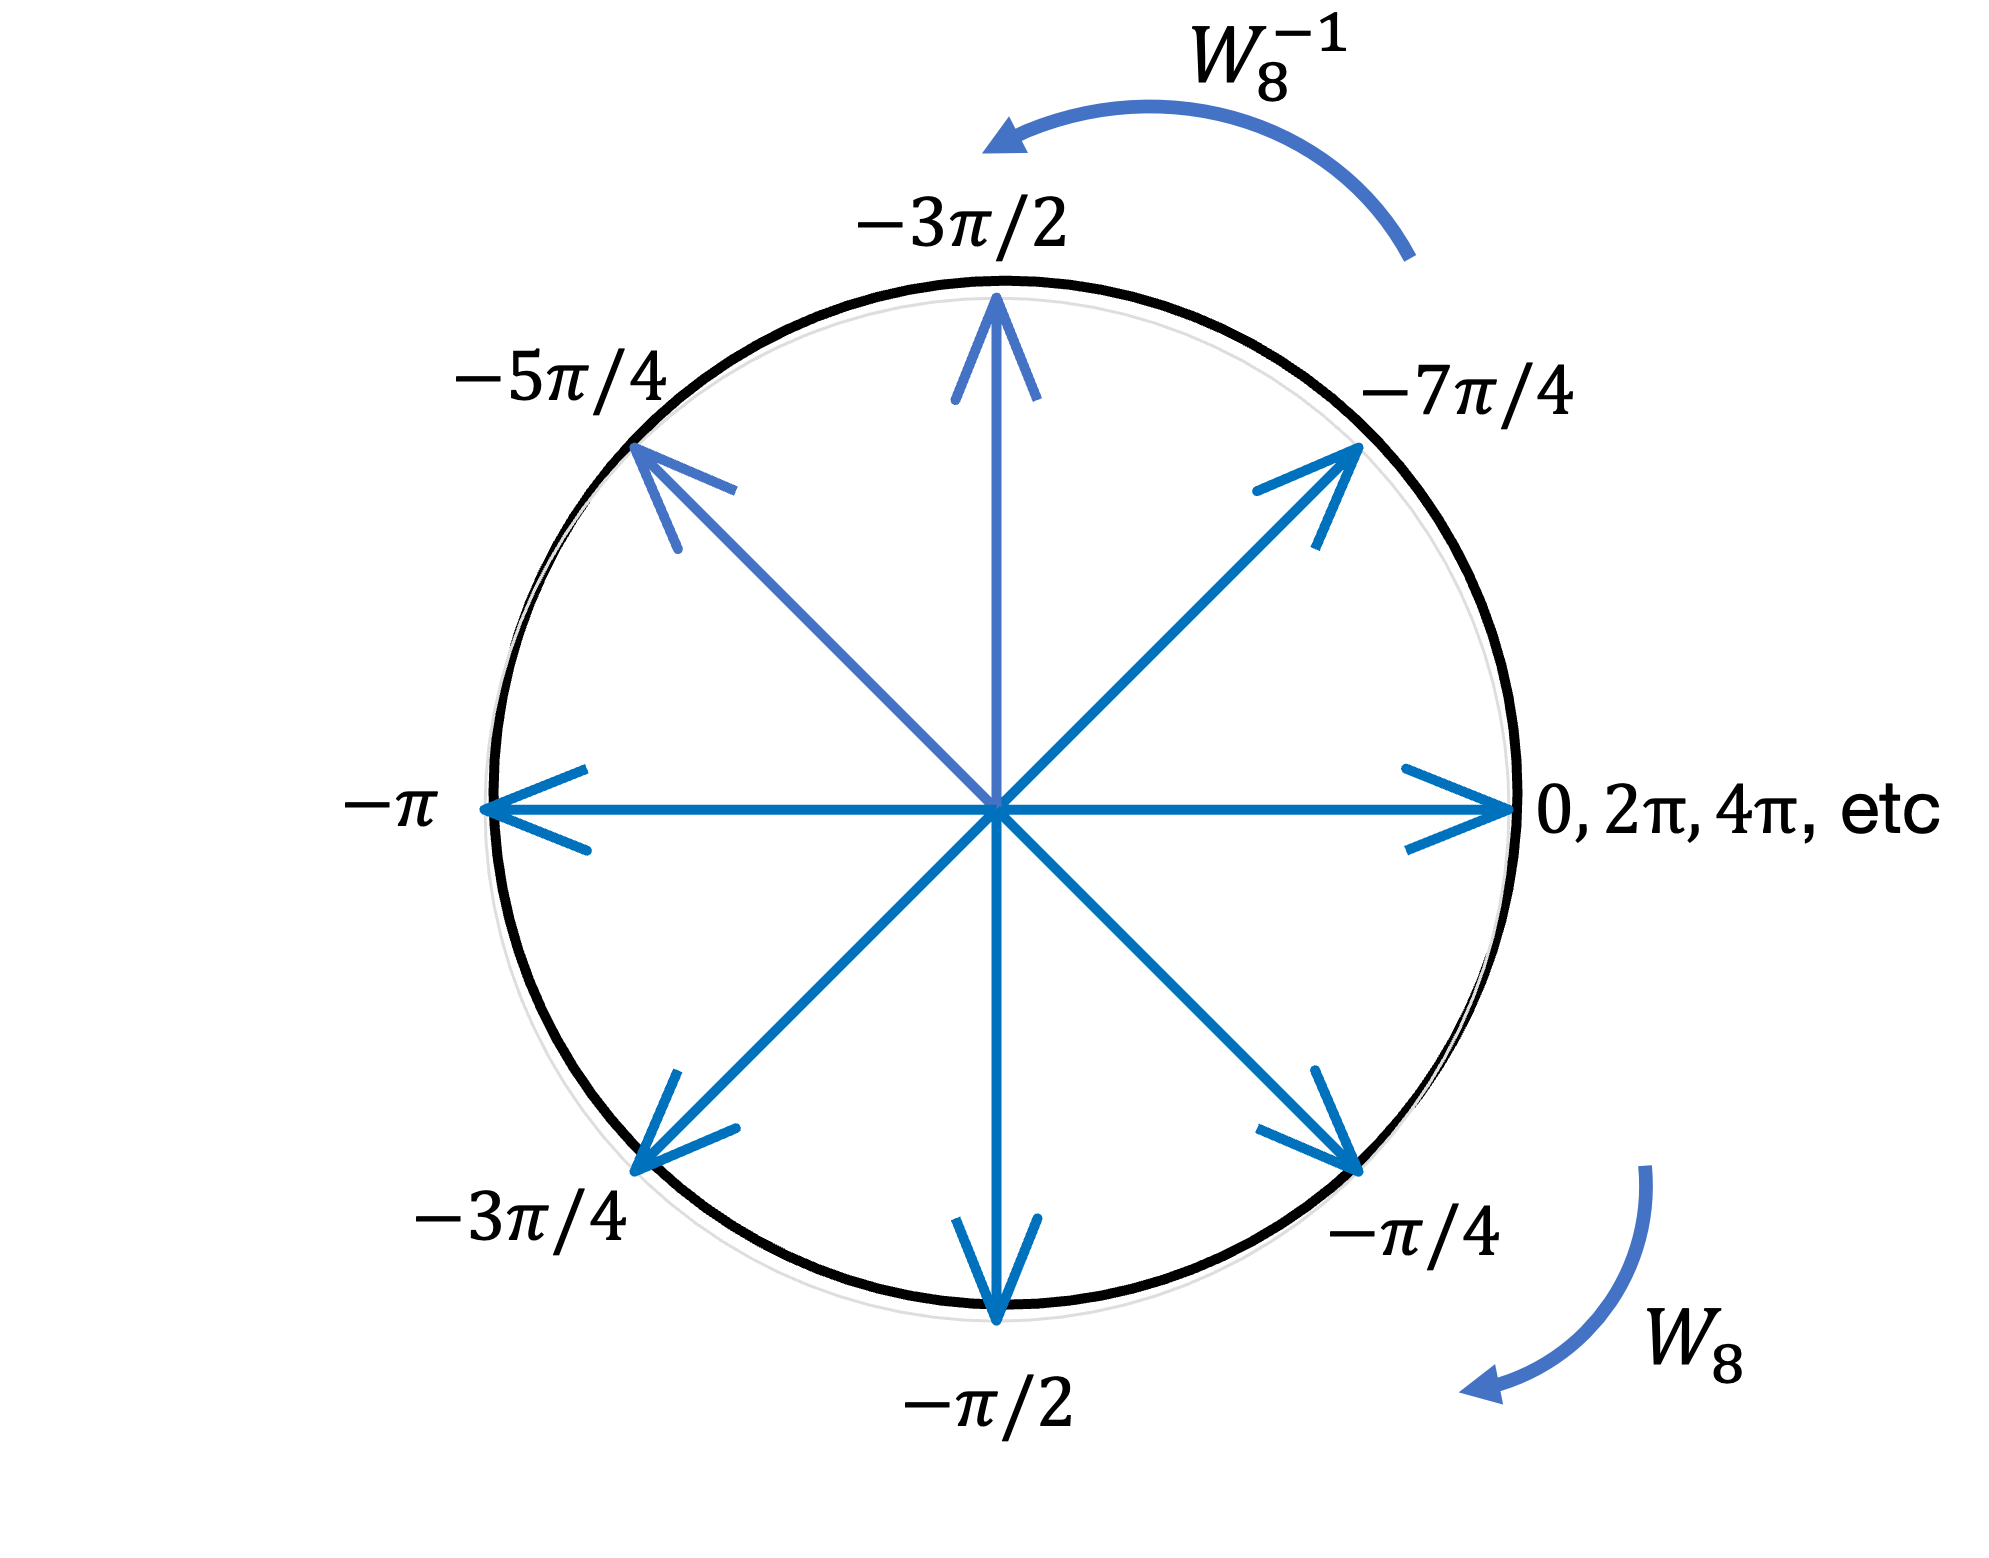
\includegraphics[width=0.5\textwidth]{formula-sheets/w_wheel.png}
            \caption{\label{fig:w_wheel} The function $W_8$ and $W_8^{-1}$}
        \end{center}
    \end{figure}



\subsubsection*{The Discrete Fourier Transform}

$$
X[m] = \sum_{n=0}^{N-1} x[n] W_N^{nm}
$$
where $W_N = \exp\left(-\frac{j2\pi}{N}\right)$.

\subsubsection*{The Inverse Discrete Fourier Transform}

$$
x[n] = \sum_{m=0}^{N-1}  x[m]W_N^{-nm}
$$
where $W_N^{-1}=\exp\left(\frac{j2\pi}{N}\right)$.

\subsection*{The function $W_N$}

$$
W_N = \exp\left(\frac{j2\pi}{N}\right) %
     = \cos\left(\frac{2\pi}{N}\right)+j\sin\left(\frac{2\pi}{N}\right)
$$
The functions $W_N$ and $W_N^{-1}$ are illustrated in Fig.~\ref{fig:w_wheel} for $N = 8$.

\endinput



\begin{center}
    \vspace*{10mm}
    \large{\textbf{End of Formulae for Examination Use}}
\end{center}


%BEGIN DO NOT EDIT
\finalize 
\label{last-page}
\end{document}
% END DO NOT EDIT


